\documentclass[aspectratio=169]{beamer} % O parâmetro aspectratio com valar 16:9 deixa o slide em widescreen

\usepackage[brazil]{babel}
\usepackage[utf8]{inputenc}
\usepackage[T1]{fontenc}

\usetheme{Madrid}
\setbeamertemplate{navigation symbols}{}

\title[Educação em Tecnologias Digitais]{Educação em Tecnologias Digitais}

\author[Diego S. C. Nascimento]{Diego Silveira Costa Nascimento}

\institute[IFRN]{
Instituto Federal de Educação, Ciência e Tecnologia do Rio Grande do Norte\\
diego.nascimento@ifrn.edu.br
}

\date[\today]{\today}

\begin{document}

\begin{frame}[plain]
	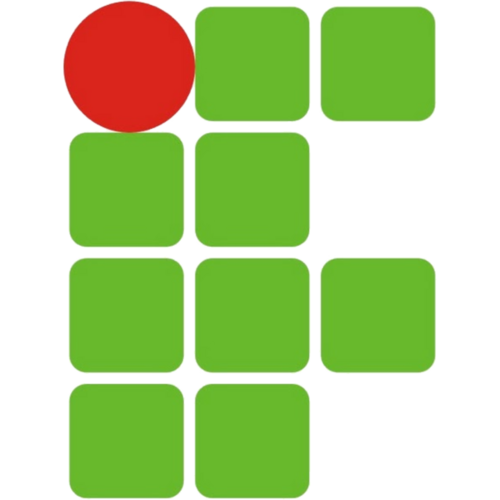
\includegraphics[scale=0.2]{img/IFRN}
	\titlepage
\end{frame}

\logo{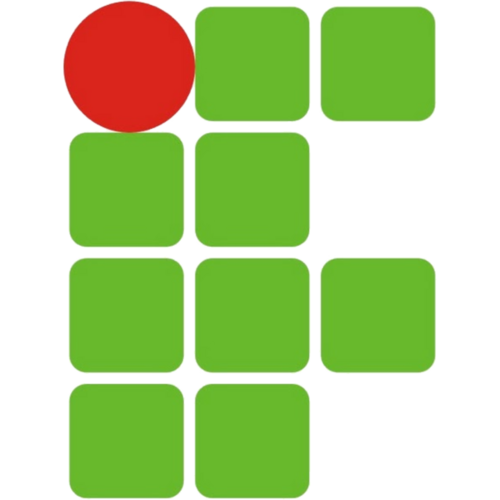
\includegraphics[scale=0.1]{img/IFRN}}

\begin{frame}
	\frametitle{Ementa do Curso}
  	\tableofcontents
\end{frame}

\AtBeginSection[]{
	\begin{frame}
		\frametitle{Ementa}
		\tableofcontents[currentsection]
	\end{frame}
}

\section{Sistemas Operacionais}

\begin{frame}
	\frametitle{Sistema Operacional}
	
	\begin{block}{Definição}
		É um programa ou um conjunto de programas cuja função é gerenciar os recursos do sistema, fornecendo uma interface entre o computador e o usuário.	
	\end{block}\vfill
	
	\begin{exampleblock}{Exemplos}
		\begin{itemize}
			\item Windows;
			\item Linux;
			\item MacOS;
			\item Chrome OS; 
			\item Android; e
			\item IOS.
		\end{itemize}
	\end{exampleblock}
\end{frame}

\begin{frame}
	\frametitle{Principais Funções}
	
	\begin{itemize}
		\item Gerenciamento de processos;
		\item Gerenciamento de memória;
		\item Gerenciamento de recursos;
		\item Entrada e saída de dados; e
		\item Sistema de arquivos.
	\end{itemize}
\end{frame}

\begin{frame}
	\frametitle{Windows}
	
	\begin{itemize}
		\item Teve a primeira versão lançada em 1985; e
		\item É uma família de sistemas operacionais comercializados e vendidos pela Microsoft.
	\end{itemize}\vfill
	
	\begin{center}
		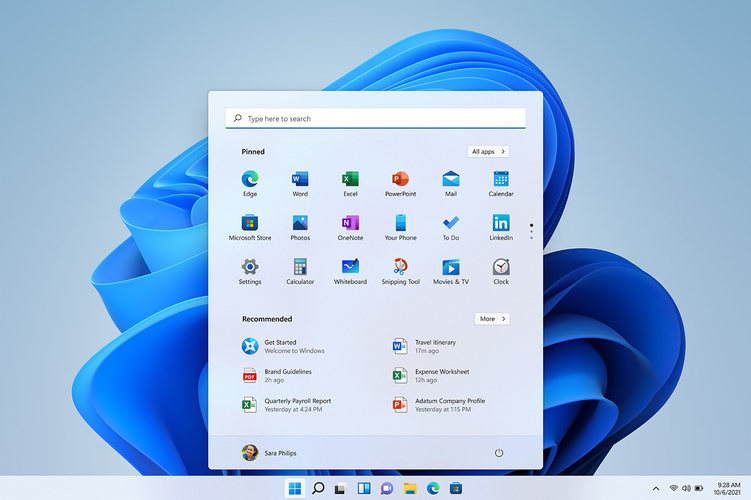
\includegraphics[scale=1]{img/windows11}
	\end{center}
\end{frame}

\begin{frame}
	\frametitle{Linux}
	
	\begin{itemize}
		\item Foi desenvolvido pelo programador finlandês Linus Torvalds, inspirado no sistema Minix; 
		\item Teve a primeira versão lançada em 1991; e
		\item O código-fonte está disponível sob a licença GPL (versão 2) para que qualquer pessoa o possa utilizar, estudar, modificar e distribuir livremente.
	\end{itemize}\vfill
	
	\begin{center}
		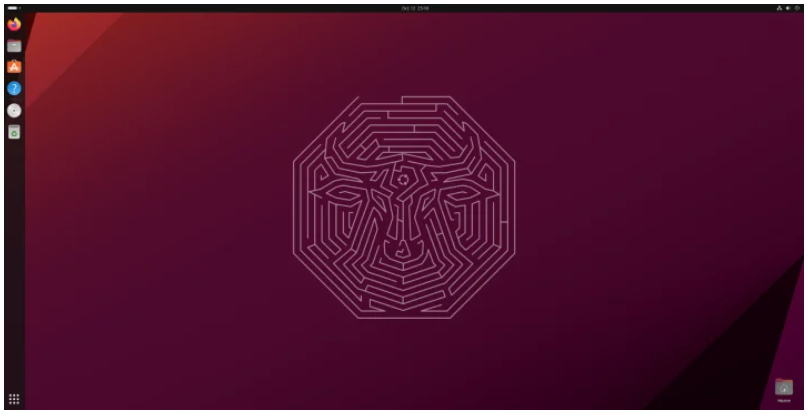
\includegraphics[scale=0.4]{img/ubuntu2310}
	\end{center}
\end{frame}

\begin{frame}
	\frametitle{MacOS}
	
	\begin{itemize}
		\item É um sistema operacional proprietário desenvolvido e distribuído pela Apple;
		\item Teve a primeira versão lançada em 1984.
	\end{itemize}\vfill
	
	\begin{center}
		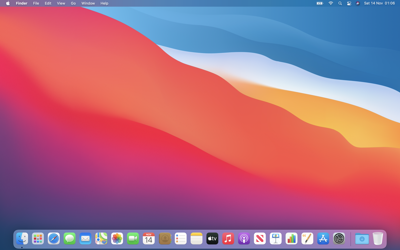
\includegraphics[scale=0.45]{img/macosbig}
	\end{center}
\end{frame}

\begin{frame}
	\frametitle{Chrome OS}
	
	\begin{itemize}
		\item É um sistema operacional desenvolvido pelo Google;
		\item Teve a primeira versão lançada em 2010; e
		\item É baseado no núcleo do Linux. 
	\end{itemize}\vfill
	
	\begin{center}
		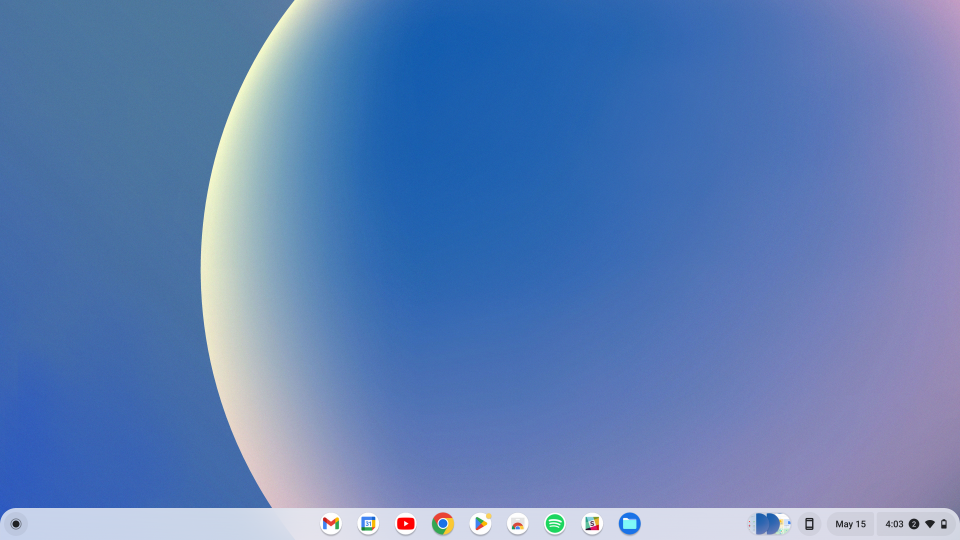
\includegraphics[scale=0.2]{img/chromeos}
	\end{center}
\end{frame}

\begin{frame}
	\frametitle{Android}
	
	\begin{itemize}
		\item Desenvolvido por um consórcio de desenvolvedores conhecido como Open Handset Alliance, sendo o principal colaborador o Google;
		\item Projetado principalmente para dispositivos móveis;
		\item Teve a primeira versão lançada em 2008; e
		\item É baseado no núcleo do Linux. 
	\end{itemize}\vfill
	
	\begin{center}
		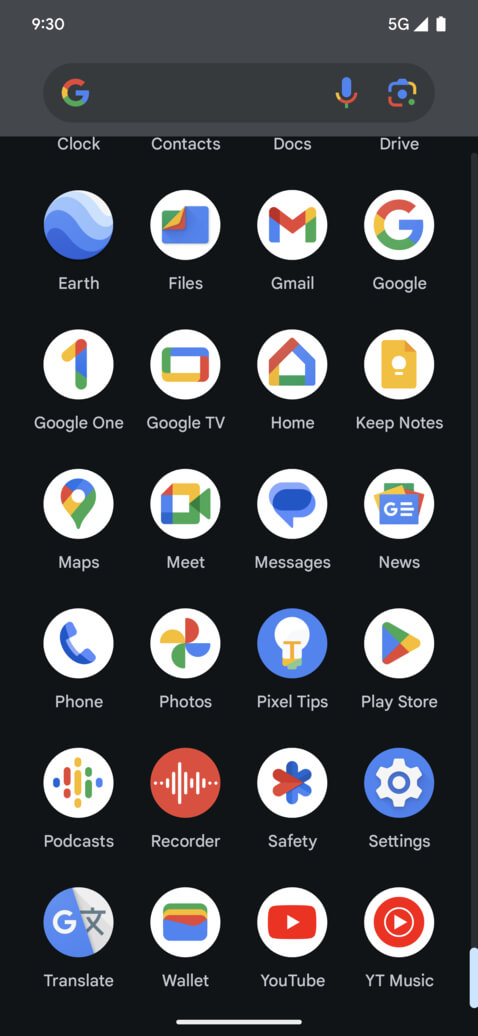
\includegraphics[scale=0.13]{img/android}
	\end{center}
\end{frame}

\begin{frame}
	\frametitle{IOS}
	
	\begin{itemize}
		\item Desenvolvido pela Apple;
		\item Projetado para dispositivos móveis; e
		\item Teve a primeira versão lançada em 2007.
	\end{itemize}\vfill
	
	\begin{center}
		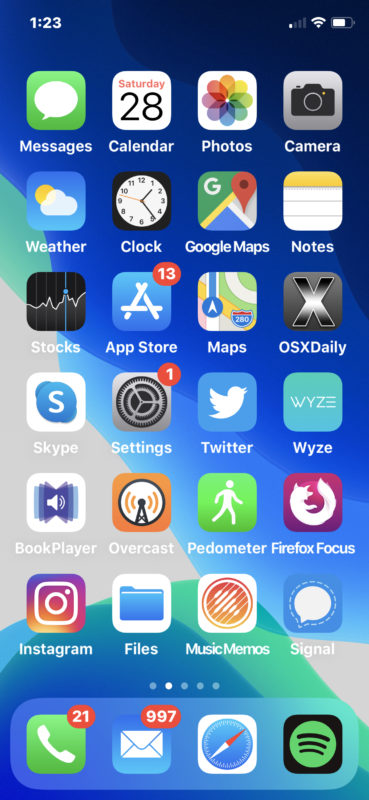
\includegraphics[scale=0.15]{img/ios}
	\end{center}
\end{frame}

\begin{frame}
	\frametitle{Usando um Sistema Operacional}
	
	\begin{itemize}
		\item Área de trabalho;
		\item Menu de programas;
		\item Barra de tarefas;
		\item Lixeira.
	\end{itemize}
\end{frame}

\begin{frame}
	\frametitle{Janela}
	
	\begin{itemize}
		\item Barra de título;
		\item Menu;
		\item Minimizar;
		\item Maximizar/Restaurar; e
		\item Fechar.
	\end{itemize}
\end{frame}

\begin{frame}
	\frametitle{Gerenciador de Arquivos}
	
	\begin{block}{Definição}
		 É um programa de computador usado para criar e organizar diretórios e arquivos em sistemas operacionais.
	\end{block}
	
	\begin{center}
		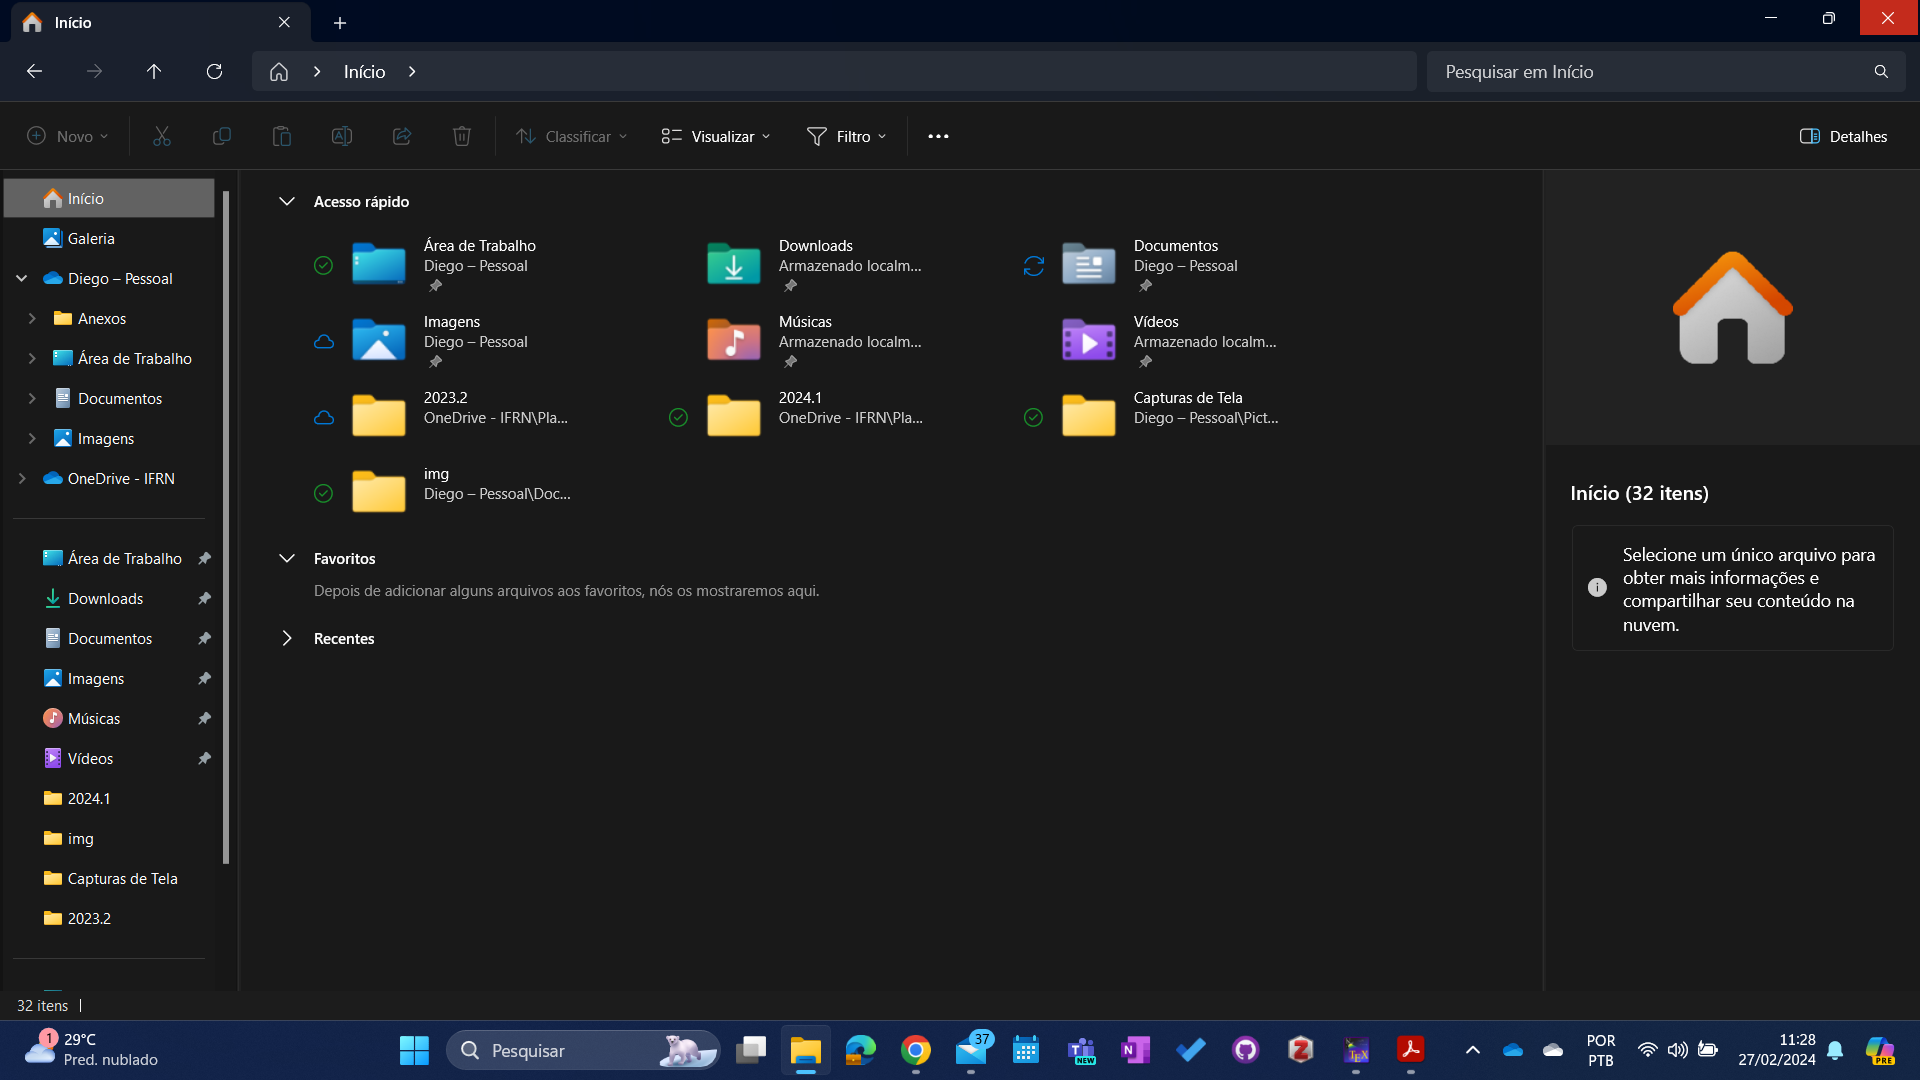
\includegraphics[scale=0.1]{img/explorador-de-arquivos}
	\end{center}
\end{frame}

\begin{frame}
	\frametitle{Configura\c cões do Sistema}
	
	\begin{itemize}
		\item Aparência; e
		\item Idioma;
		\item Contas da internet;
		\item Impressora;
		\item Teclado;
		\item Mouse;
		\item Atualiza\c cões do sistema; e
		\item Instala\c cão de programas.
	\end{itemize}
\end{frame}

\begin{frame}
	\frametitle{Encerramento do Sistema}
	
	\begin{itemize}
		\item Suspender;
		\item Reiniciar; e
		\item Desligar.
	\end{itemize}
\end{frame}

\begin{frame}
	\frametitle{Softwares Utilitários}
	
	\begin{block}{Defini\c cão}
		São software projetados para fornecer funcionalidades adicionais e recursos que não são encontrados nos sistemas operacionais padrão.
	\end{block}\vfill
	
	\begin{exampleblock}{Exemplos}
		\begin{itemize}
			\item Compactadores;
			\item Antivírus;
			\item Backup; e
			\item Desfragmentador de disco.
		\end{itemize}
	\end{exampleblock}
\end{frame}

\begin{frame}
	\frametitle{Compacta\c cão de Arquivos}
	
	\begin{block}{Defini\c cão}
		São softwares especializados em gerar uma representação mais eficiente de vários arquivos dentro de um único arquivo, de modo que ocupem menos espaço na mídia de armazenamento.
	\end{block} \vfill
	
	\begin{exampleblock}{Exemplos}
		\begin{itemize}
			\item 7-Zip;
			\item WinZip; e
			\item WinRAR.
		\end{itemize}
	\end{exampleblock}
\end{frame}

\begin{frame}
	\frametitle{Antivírus}
	
	\begin{block}{Defini\c cão}
		É um programa utilizado para prevenir, detectar e eliminar malwares e vírus.
	\end{block}\vfill

	\begin{exampleblock}{Programas}
		\begin{itemize}
			\item McAfee;
			\item Microsoft Defender;
			\item Avast;
			\item AVG.
		\end{itemize}
	\end{exampleblock}
\end{frame}

\begin{frame}
	\frametitle{Backup}
	
	\begin{block}{Defini\c cão}
		É um termo utilizado para uma atividade que consiste em realizar cópias de segurança de dados digitais de um dispositivo com o intuito de recuperá-los em caso de perdas acidentais ou falhas no sistema em que os arquivos estão armazenados.
	\end{block}
\end{frame}

\begin{frame}
	\frametitle{Desfragmentador de Arquivos}
	
	\begin{block}{Defini\c cão}
		É uma ferramenta que permite analisar o desfragmentar unidades de disco, tornando o computador mais rápido, eficiente e ganhando velocidade.
	\end{block}\vfill
	
	\begin{center}
		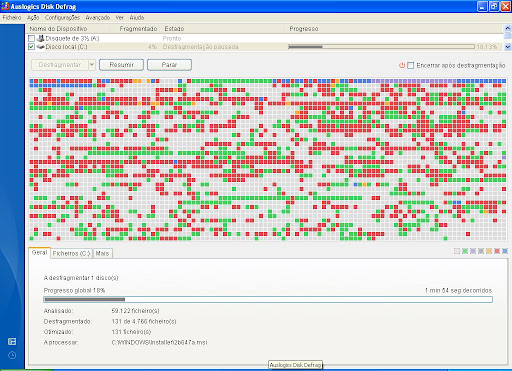
\includegraphics[scale=0.4]{img/desfragmentador}
	\end{center}
\end{frame}

\section{Internet}

\begin{frame}
	\frametitle{Internet}
	
	\begin{block}{Defini\c cão}
		É uma rede global de dispositivos interconectados que permite a comunicação instantânea e o acesso a uma vasta quantidade de informações.
	\end{block}
\end{frame}

\begin{frame}
	\frametitle{Como Funciona?}
	
	\begin{itemize}
		\item A Internet funciona por meio de protocolos de comunicação;
		\item O protocolo padrão é o TCP/IP;
		\item Os dados são transmitidos por meio de roteadores e servidores em todo o mundo; e
		\item Os dados são transmitido por meio de pacotes.
	\end{itemize}
\end{frame}

\begin{frame}
	\frametitle{Benefícios}
	
	\begin{itemize}
		\item Acesso à informação em tempo real;
		\item Comunicação fácil e instantânea; e
		\item Compartilhamento de recursos e colaboração global.
	\end{itemize}
\end{frame}

\begin{frame}
	\frametitle{História}
	
	\begin{itemize}
		\item Início da década de 1960: a partir de pesquisas militares, no períodos, da Guerra Fria, começam a surgir os primeiros esboços da internet;
		\item 1969: DARPA (Department Advanced Reseach and Projects Agency) patrocinou o projeto que mais tarde seria chamado ARPANET;
		\item Início de 1983: ARPANET adota o protocolo TCP/IP;
		\item 1985: NSF (National Science Foundation) interliga seus supercomputadores formando a NSFnet.
		\item 1986: NSFnet conecta-se ao ARPANET e passa a ser chamada de Internet;
		\item 1989: Comunidade acadêmica Rio-São Paulo (Fadesp + LNCC/UFRJ) se liga a Internet;
	\end{itemize}
\end{frame}

\begin{frame}
	\frametitle{História}
	
	\begin{itemize}
		\item 1992: O cientista Tim Berners-Lee, do CERN, criou a World Wide Web – www;
		\item 1993: A Internet passa a ser explorada comercialmente no EUA e em outros países;
		\item A Internet tem seu sucesso fora do mundo acadêmico graças à distribuição do Mosaic, o primeiro navegador para a Web; e
		\item 1994: A Internet passa a ser explorada comercialmente no Brasil; e Sai a primeira versão do Netscape Navigator.
	\end{itemize}
\end{frame}

\begin{frame}
	\frametitle{O que é uma página?}
	
	\begin{block}{Defini\c cão}
		É uma coleção específica de informações (textos, imagens, vídeos, e outros arquivos multimídia) fornecidas por um site e exibidas a um usuário em um navegador web.
	\end{block} \vfill

	\begin{center}
		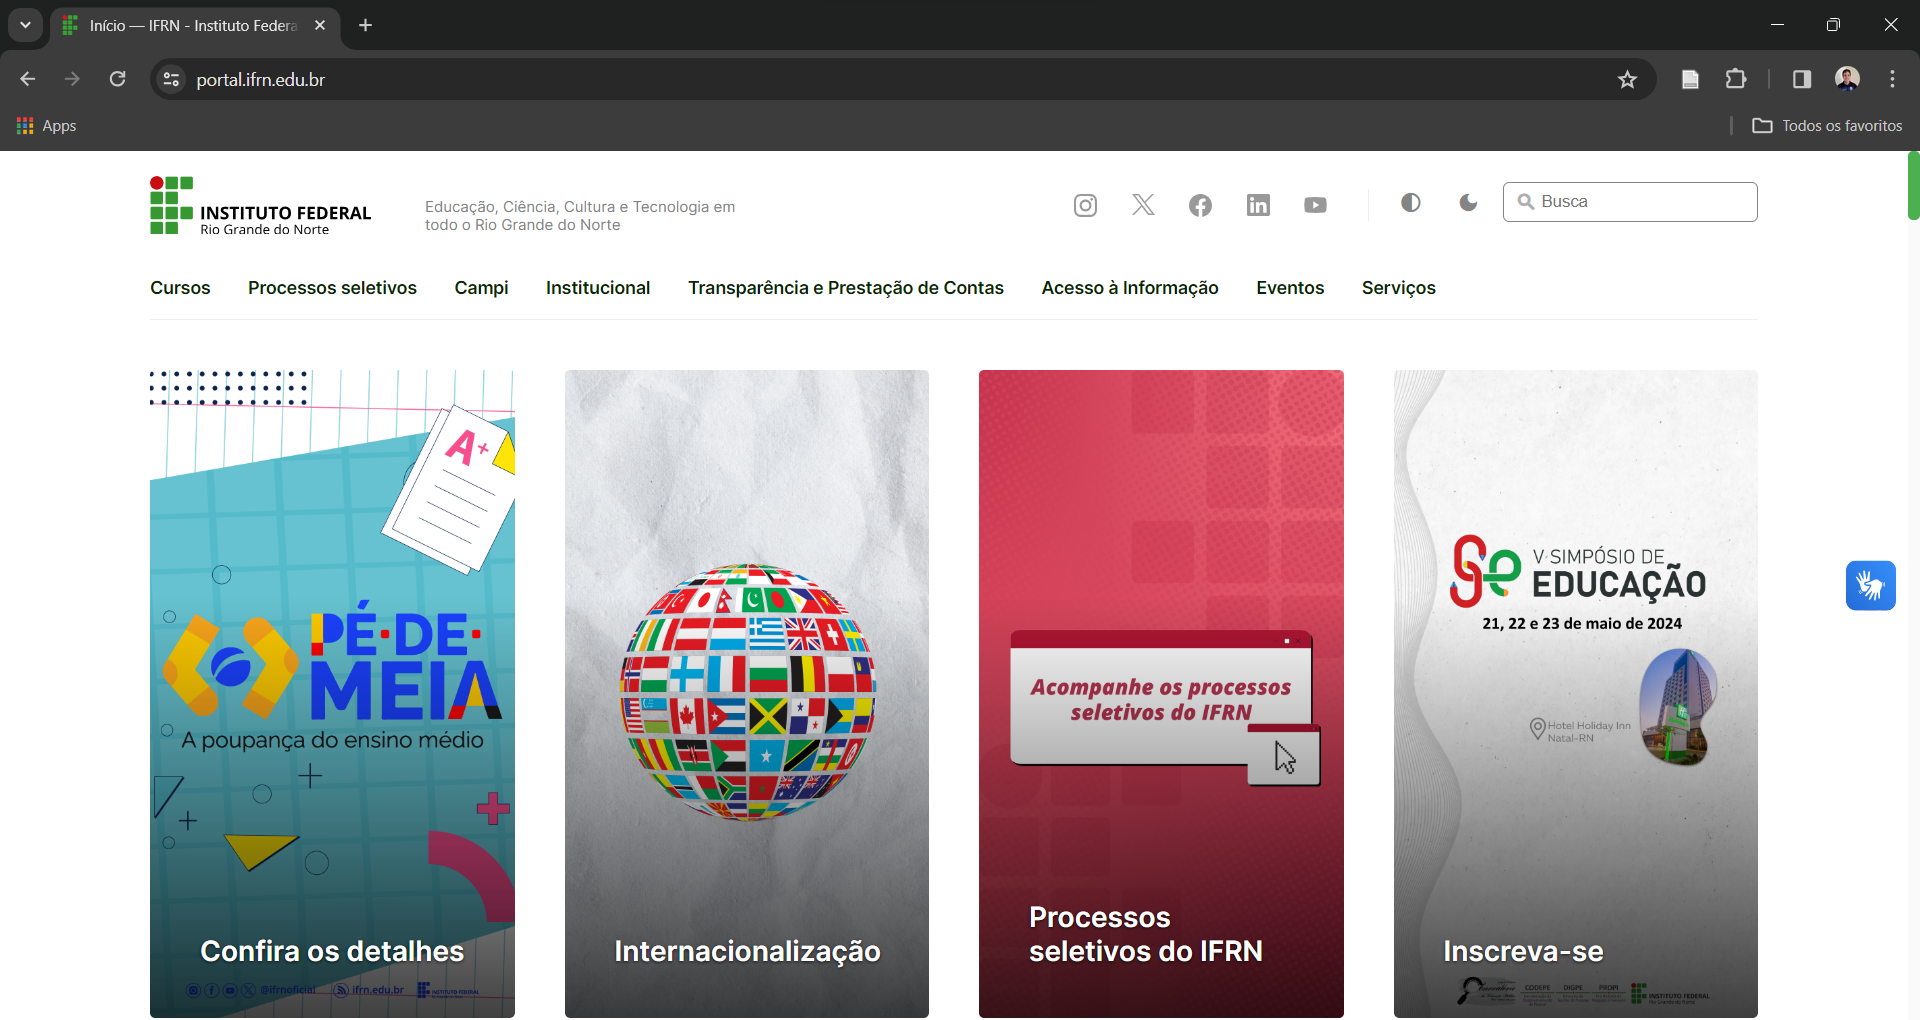
\includegraphics[scale=0.13]{img/pagina}
	\end{center}
\end{frame}

\begin{frame}
	\frametitle{O que é URL?}
	
	\begin{block}{Defini\c cão}
		É o endereço virtual de uma página ou website.
	\end{block} \vfill
	
	\begin{itemize}
		\item Um acrônimo para \underline{U}niform \underline{R}esource \underline{L}ocator;
		\item Está divida em: 
		\begin{enumerate}
			\item Protocolo; 
			\item Subdomínio;
			\item Domínio; e 
			\item Subdiretórios.
		\end{enumerate}				
	\end{itemize} \vfill
	
	\begin{exampleblock}{Exemplo}
		\begin{center}
			$\underbrace{http}_{1}$://$\underbrace{www}_{2}$.$\underbrace{ifrn.edu.br}_{3}$/$\underbrace{cal}_{4}$
		\end{center}
	\end{exampleblock}
\end{frame}

\begin{frame}
	\frametitle{Navegador}
	
	\begin{block}{Defini\c cão}
		É um programa que habilita seus usuários a interagirem com documentos HTML hospedados em um servidor da rede.
	\end{block} \vfill
	
	\begin{exampleblock}{Exemplos}
		\begin{itemize}
			\item Google Chrome;
			\item Mozilla Firefox;
			\item Microsoft Egde;
			\item Safari;
			\item Opera; e
			\item Brave.
		\end{itemize}
	\end{exampleblock}
\end{frame}

\begin{frame}
	\frametitle{Entendendo o Navegador}
	
	\begin{itemize}
		\item Barra de endereço;
		\item Abas;
		\item Favoritos; e
		\item Janela anônima.
	\end{itemize}
\end{frame}

\begin{frame}
	\frametitle{Correio Eletrônico}
	
	\begin{block}{Defini\c cão}
		É uma tecnologia que permite compor, enviar e receber mensagens através de sistemas eletrônicos de comunicação assíncrona.
	\end{block}
\end{frame}

\begin{frame}
	\frametitle{O que é endere\c co de e-mail?}
	
	\begin{block}{Defini\c cão}
		É o endere\c co postal na internet.
	\end{block} \vfill
	
	\begin{itemize}
		\item Está divida em: 
		\begin{enumerate}
			\item Nome do utilizador; 
			\item Símbolo;  e
			\item Domínio. 
		\end{enumerate}				
	\end{itemize} \vfill
	
	\begin{exampleblock}{Exemplo}
		\begin{center}
			$\underbrace{exemplo}_{1}$ $\underbrace{@}_{2}$ $\underbrace{ifrn.edu.br}_{3}$
		\end{center}
	\end{exampleblock}
\end{frame}

\begin{frame}
	\frametitle{Organiza\c cão do correio eletrônico}
	
	\begin{itemize}
		\item Caixa de entrada;
		\item Enviados;
		\item Rascunhos;
		\item Excluídos; e
		\item Spam.
	\end{itemize}
\end{frame}

\begin{frame}
	\frametitle{Composi\c cão da Mensagem}
	
	\begin{itemize}
		\item Destinatário;
		\item Assunto;
		\item Corpo do e-mail; e
		\item Anexos.
	\end{itemize}
\end{frame}

\begin{frame}
	\frametitle{Armazenamento em Nuvem}
	
	\begin{block}{Defini\c cão}
		É um serviço de armazenamento e sincronização de arquivos a partir de qualquer computador ou outros dispositivos compatíveis ligados à internet.
	\end{block} \vfill
	
	\begin{exampleblock}{Exemplos}
		\begin{itemize}
			\item Google Drive;
			\item OneDrive;
			\item iCloud; 
			\item Dropbox; e
			\item Amazon Cloud.
		\end{itemize}
	\end{exampleblock}
\end{frame}

\begin{frame}
	\frametitle{Utilizando o armazenamento em nuvem}
	
	\begin{itemize}
		\item Criando/Carregando pasta;
		\item Criando/Carregando arquivo; e
		\item Realizando compartilhamento.
	\end{itemize}
\end{frame}

\begin{frame}
	\frametitle{Ambiente Virtual de Aprendizagem}
	
	\begin{block}{Definição}
		 É uma plataforma baseada na web para os aspectos digitais dos cursos de estudo, geralmente dentro de instituições educacionais.
	\end{block}
\end{frame}

\begin{frame}
	\frametitle{Principais Recursos do AVA}
	
	\begin{itemize}
		\item Plataforma de cursos online;
		\item Fóruns de discussão;
		\item Videoaulas e materiais didáticos;
		\item Chat e mensagens instantâneas;
		\item Ferramentas de avaliação (testes, questionários, provas online).
	\end{itemize}
\end{frame}

\begin{frame}
	\frametitle{Benefícios do AVA}
	
	\begin{itemize}
		\item Acessibilidade: possibilita o acesso ao conteúdo a qualquer momento e de qualquer lugar;
		\item Flexibilidade: permite o aprendizado em um ritmo personalizado;
		\item Interação e colaboração: facilita a comunicação entre alunos e professores, além da troca de experiências entre os próprios alunos;
		\item Diversidade de recursos: oferece diferentes formatos de conteúdo para atender às necessidades dos alunos.
	\end{itemize}
\end{frame}

\begin{frame}
	\frametitle{Segurança da Informação}
	
	\begin{block}{Definição}
		 É uma série de ações adotadas estrategicamente para controlar e evitar riscos de roubo, danos e perdas dos dados, dispositivos, servidores, sistemas e redes.
	\end{block}
\end{frame}

\begin{frame}
	\frametitle{Pilares da Segurança da Informação}

	\begin{itemize}
		\item Confiabilidade;
		\item Integridade; e
		\item Disponibilidade.
	\end{itemize}
\end{frame}

\begin{frame}
	\frametitle{Ameaças à Segurança da Informação}
	
	\begin{itemize}
		\item Malware;
		\item Phishing;
		\item Ataques de DDoS; e
		\item Engenharia Social.
	\end{itemize}
\end{frame}

\begin{frame}
	\frametitle{Práticas de Segurança da Informação}
	
	\begin{itemize}
		\item Senhas fortes;
		\item Autenticação de dois fatores;
		\item Atualizações regulares de software;
		\item Backup regular de dados; e
		\item Políticas de controle de acesso.
	\end{itemize}
\end{frame}

\begin{frame}
	\frametitle{Regulamentação}
	
	\begin{itemize}
		\item Lei Geral de Proteção de Dados (LGPD) no Brasil;
		\item Lei n$^{\circ}$ 13.709/2018 de 14 de agosto de 2018; e
		\item Controla a privacidade e o uso/tratamento de dados pessoais.
	\end{itemize}
\end{frame}

\begin{frame}
	\frametitle{Princípios da LGPD}
	
	\begin{itemize}
		\item Finalidade;
		\item Adequação;
		\item Necessidade;
		\item Livre Acesso;
		\item Transparência;
		\item Segurança;
		\item Prevenção; e
		\item Não Discriminação.
	\end{itemize}
\end{frame}

\begin{frame}
	\frametitle{Direitos dos Titulares de Dados}
	
	\begin{itemize}
		\item Direito de acesso;
		\item Direito de retificação;
		\item Direito à exclusão;
		\item Direito à portabilidade; e
		\item Direito à revogação do consentimento.
	\end{itemize}
\end{frame}

\begin{frame}
	\frametitle{Penalidades}
	
	\begin{itemize}
		\item 2$\%$ do faturamento da companhia;
		\item Limitado até 50 milhões;
		\item Retratação pública; e
		\item Reparação dos danos as pessoas afetadas.
	\end{itemize}
\end{frame}

\section{Inteligência Artificial na Educação}

\begin{frame}
	\frametitle{Inteligência Artificial}
	
	\begin{block}{Definição}
		É  o estudo que permite desenvolver máquinas com capacidade de  aprender com experiências, se adaptar a diferentes situações e realizar tarefas que normalmente exigiriam características ou respostas inteligentes.
	\end{block}
\end{frame}

\begin{frame}
	\frametitle{Aplicações de IA}
	
	\begin{itemize}
		\item Assistentes virtuais;
		\item Recomendações personalizadas;
		\item Reconhecimento facial;
		\item Tradução automática;
		\item Detecção de fraudes;
		\item Carros autônomos; e
		\item Diagnóstico médico.
	\end{itemize}
\end{frame}

\begin{frame}
	\frametitle{Benefícios da IA na Educação}
	
	\begin{itemize}
		\item Personalização da aprendizagem;
		\item Tutoria virtual e assistência aos alunos;
		\item Análise preditiva para identificar necessidades dos alunos; e
		\item Automatização de tarefas administrativas.
	\end{itemize}
\end{frame}

\begin{frame}
	\frametitle{Aplicações Práticas de IA na Educação}
	
	\begin{itemize}
		\item Sistemas de recomendação de conteúdo educacional;
		\item Plataformas de ensino adaptativo;
		\item Avaliação automatizada de desempenho dos alunos; e
		\item Ferramentas de tradução e interpretação em tempo real.
	\end{itemize}
\end{frame}

\section{Editor de Texto}

\section{Editor de Apresentação}

\section{Editor de Planilha Eletrônica}

\end{document}